\documentclass[12pt]{article}
\usepackage[spanish]{babel}
\usepackage[utf8]{inputenc}
\usepackage{csquotes}

% Interlineado 1.5
\usepackage{mathpazo}
\usepackage{setspace}
\onehalfspacing

% Fuente Times New Roman
\usepackage{mathptmx}

% Acomodar margenes del documento
\usepackage[a4paper, margin=2cm, top=3cm, headheight=50pt]{geometry}

% Paquetes comunes
\usepackage{graphicx, float}
\usepackage{amsfonts, amssymb, amsmath}
\usepackage{physics, esvect}
\usepackage{enumerate}
\usepackage[colorlinks=true, citecolor=blue]{hyperref}

% Para graficar
\usepackage{pgfplots}
\usepackage{tikz, color}
\usepackage{tikz-3dplot}
\pgfplotsset{width=15cm, compat=1.18}
\usepgfplotslibrary{external}
\tikzexternalize[prefix=figs/]

% Para automatas
\usetikzlibrary{automata, positioning, arrows, calc}
\tikzset{
        ->,  % makes the edges directed
        >=stealth, % makes the arrow heads bold
        shorten >=2pt, shorten <=2pt, % shorten the arrow
        node distance=3cm, % specifies the minimum distance between two nodes. Change if n
        every state/.style={draw=blue!55,very thick,fill=blue!20}, % sets the properties for each ’state’ n
        initial text=$ $, % sets the text that appears on the start arrow
}

% Encabezados
\usepackage{fancyhdr}
\pagestyle{fancy}
\fancyhf{}
\fancyfoot[C]{\thepage}
\fancyhead[L]{
  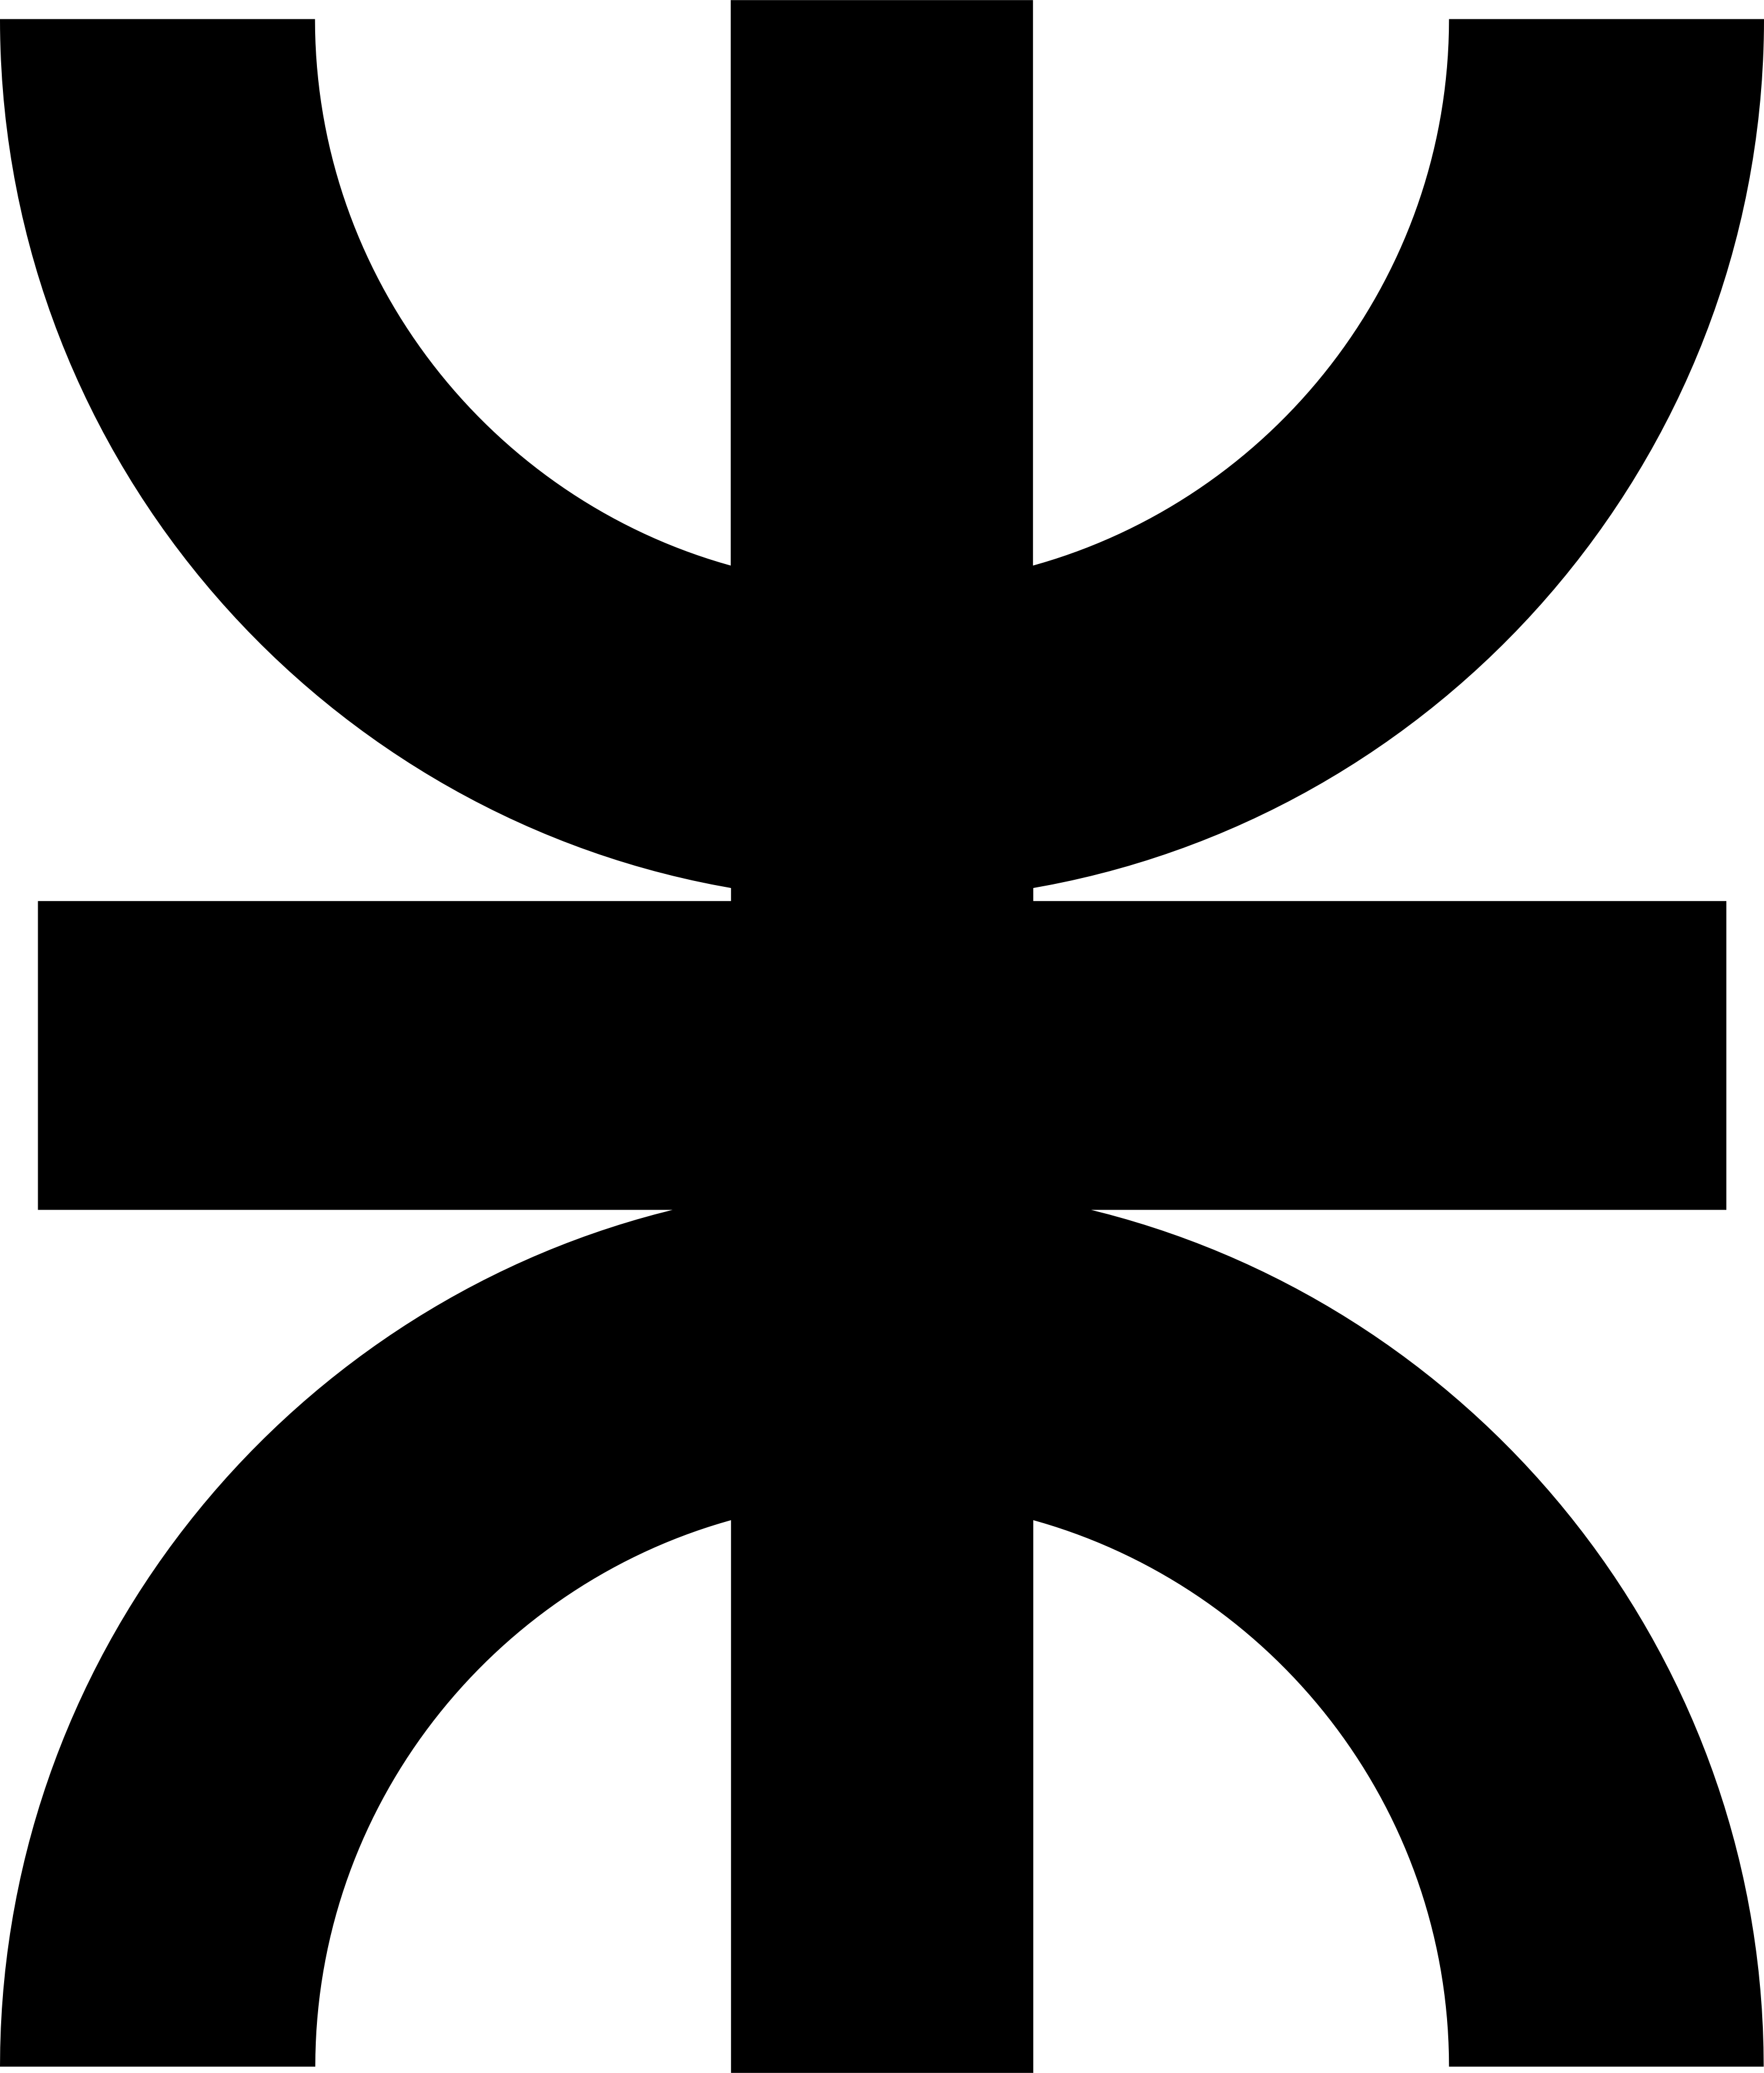
\includegraphics[height=1.2cm]{~/imagenes/logo_utn.png}
  \shortstack[l]{
    {\footnotesize Universidad Tecnológica Nacional} \\
    {\footnotesize Facultad Regional Córdoba} \\
    {\footnotesize Extensión Áulica Bariloche}
  }
}
\fancyhead[C]{
  \shortstack[c]{
    {\footnotesize Física 2} \\
    {\footnotesize Proyecto N° 1} \\
    {\footnotesize }
  }
}
\fancyhead[R]{
  \shortstack[r]{
    {\footnotesize Profesor: Santiago Ibañez} \\
    {\footnotesize Alumno: Ricardo Nicolás Freccero} \\
    {\footnotesize Fecha: 14/08/2025}
  }
}

% Para bibliografía
%\usepackage[backend=biber, style=apa]{biblatex}
%\addbibresource{bibliografia.bib}

\begin{document}
\newgeometry{margin=2cm, top=1.5cm}
\begin{titlepage}
  \centering
  
\includegraphics[width=\linewidth]{~/imagenes/logo_utn_frc.jpg}\\

  \textsc{
    \LARGE Universidad Tecnológica Nacional\\
    \Large Facultad Regional Córdoba - Extensión Áulica Bariloche\\
    \large Ingeniería en Sistemas de Información\\
    Año lectivo 2025\\[0.5cm]
  }

  \rule{\linewidth}{1.0mm}\\[0.4cm]
  \Huge
  \textbf{Física 2}\\
  Proyecto N° 1\\[0.2cm]
  \LARGE
  Generador de Van de Graaff
  \rule{\linewidth}{1.0mm}\\
  \large
  \begin{flushleft}
    Profesor: Santiago Ibañez

    Ayudante: Leandro

    Fecha: 14/08/2025
  \end{flushleft}

  \vfill
  \begin{flushright}
    Alumno: Ricardo Nicolás Freccero

    Número de legajo: 415753
  \end{flushright}
\end{titlepage}

\restoregeometry
\tableofcontents
\newpage

\section{Presentación}
\subsubsection*{Portada}
Buenas tardes. Somos Ricardo Freccero y Camila Leveratto, y hoy les presentamos el proyecto de Física II: la construcción y análisis de un \textbf{generador de Van de Graaff}. El objetivo fue diseñar y montar un generador casero capaz de mostrar en un ambiente de laboratorio algunos conceptos de la electrostática (descargas, repulsión de objetos livianos), y analizar su funcionamiento aplicando los conceptos aprendidos durante la cursada (ley de Coulomb, ley de Gauss, flujo, potencial, etc.). En el informe que le entregamos al profesor describimos cómo fue el proceso de construcción, algunas observaciónes, y algún que otro cálculo con estimaciones teóricas. En esta presentación vamos a destacar los principales puntos del informe y mas que nada las cuestiones físicas y matemáticas para demostrar que aprendimos, entendimos y podemos aplicar los conceptos de la electrostática que provée la cátedra.

\subsubsection*{Índice}
Este va a ser el orden que vamos a seguir a lo largo de la presentación.
\begin{itemize}
  \item Primero vamos a hablar un poco sobre el diseño y montaje.

  \item Luego vamos a explicar cómo funciona.

  \item Una vez que entendemos cómo funciona podemos introducir la parte teórica con las derivaciones y los cálculos numéricos.

  \item Y finalmente vamos a presentar los resultados que obtuvimos con los experimentos que pudimos realizar a modo de conclusión.
\end{itemize}

\subsubsection*{Objetivos}
Los objetivos del proyecto eran principalmente dos:
\begin{itemize}
  \item Por un lado, la idea es poder visualizar fenómenos electrostáticos como chispas y repulsiones.

  \item Por otro lado, queríamos poder reproducir un dispositivo funcional que nos permita aplicar y verificar el marco teórico que vinimos desarrollando a lo largo de la cursada: ley de Coulomb, ley de Gauss, potencial eléctrico, capacidad.
\end{itemize}

\subsubsection*{¿Qué es y para qué sirve un Generador de Van de Graaff?}
El generador de Van de Graaff es un dispositivo, inventado en 1929 por R. J. Van de Graaff, diseñado para generar altos voltajes. Inicialmente fue desarrollado como una herramienta para experimentos de física de partículas. Hoy en día, es un instrumento que se usa principalmente con fines educativos para la demostración de principios electrostáticos.

Su principio es mover carga con una cinta aislante hacia una cúpula conductora donde se acumula. La acumulación de carga en este caso es una acumulación progresiva: el motor mueve la cinta, la cinta transporta carga y la esfera la almacena.

\subsubsection*{Efecto triboeléctrico y carga por inducción.}
\paragraph*{Efecto triboeléctrico}\mbox{}

Un concepto fundamental para entender cómo es que funciona este generador es el efecto triboeléctrico. El efecto triboeléctrico es la transferencia de electrones entre dos materiales cuando estos entran en contacto y luego se separan. En nuestro generador, el rodillo de teflón gana electrones (se vuelve negativo) y la cinta queda cargada positivamente. Es importante aclarar: la fricción facilita la transferencia, pero muchas veces basta con solo el contacto y la separación de los materiales. La humedad en el ambiente puede reducir la eficiencia del generador debido a fugas.

\paragraph*{Carga por inducción}\mbox{}
La carga por inducción es un proceso por el cual la presencia de una carga externa próxima a un cuerpo conductor provoca una redistribución de las cargas libres de ese conductor sin que exista contacto. El resultado es una aparición de regiones de carga neta de signo opuesto en la cara más próxima a la carga externa y de signo igual en la cara opuesta; si el conductor está puesto a tierra, las cargas de signo opuesto pueden fluir hacia tierra.

En el caso de nuestro generador, cuando la banda sube, va cargada positivamente hasta llegar al rodillo superior. Cerca del rodillo se encuentra un peine de aluminio conectado a la esfera de metal. Cuando la banda cargada pasa cerca del peine, la presencia de la carga positiva en la banda induce cargas negativas en las puntas del peine. Esta redistribución de cargas favorece el flujo de electrones entre la esfera y la banda a través del peine (en nuestro caso por ionización del aire [efecto corona], ya que el peine y la banda nunca entran en contacto), de modo que la esfera acumula carga del mismo signo que la que transporta la banda.

La banda ahora recibió una gran cantidad de electrones por parte de la esfera, y ademas esta en contacto con el rodillo superior que está hecho de nylon, por lo que va a ganar aún mas electrones provenientes del mismo. En su recorrido de vuelva al rodillo inferior entonces, la banda viaja con una carga negativa. Sin embargo, cerca del rodillo inferior se encuentra un peine conductor que está conectado a tierra. Cuando la banda llega cargada negativamente, esta induce cargas positivas en las puntas del peine: los electrones del peine son repelidos hacia tierra. Nuevamente, esta diferencia de potencial local facilita la transferencia de electrones desde la cinta hacia el peine (también por efecto corona, ya que el peine nunca entra en contacto con la banda). Los electrones fluyen por el peine hasta tierra, de modo que la cinta sale del peine cargada positivamente y se vuelve a repetir el ciclo.

\subsubsection*{Capacitores y capacitancia.}
Un capacitor es un dispositivo que almacena energía potencial eléctrica y carga eléctrica. Físicamente están compuestos por dos conductores aislados entre sí.

La capacitancia es una propiedad que mide la capacidad de un sistema para almacenar carga eléctrica por unidad de potencial eléctrico y se mide en Faradios. Un sistema con alta capacitancia puede almacenar mas carga para un mismo voltaje en comparacion con uno de baja capacitancia.

\subsubsection*{Campo eléctrico y potencial eléctrico.}
Lo que dice la ley de Coulomb es que existen algunas partículas que tienen una propiedad que se llama carga eléctrica medida en Coulombs. Además, dadas dos partículas cargadas, podemos calcular la fuerza que ejerce una sobre la otra con la siguiente fórmula.
\[
  \vv{F} = \frac{\left|q_{1}q_{2}\right|}{4\pi\varepsilon_{0}} \frac{1}{r^2} \hat{r}
\]

De esta forma, podemos decir que cada partícula cargada genera un campo eléctrico a su alrededor de la forma
\[
  \vv{E} = \frac{\left|q\right|}{4\pi\varepsilon_{0}} \frac{1}{r^2} \hat{r}
\]

\subsubsection*{Ley de Gauss y Potencial Eléctrico}
La ley de Gauss establece que el flujo eléctrico total que atraviesa una superficie cerrada depende únicamente de la carga eléctrica que esa superficie encierra. Esta ley es muy importante para física 2 ya que nos simplifica en gran medida el cálculo del campo eléctrico.

El potencial eléctrico, por otro lado, es el trabajo por unidad de carga necesario para llevar una carga de prueba desde un punto de referencia hasta otro punto. Este está relacionado con el campo eléctrico en el sentido que el campo eléctrico es menos el gradiente del potencial eléctrico. De esta manera, podemos obtener la ecuación de uno a partir del otro.

Para calcular el campo eléctrico de la esfera de nuestro generador vamos a usar la ley de Gauss. Para ello planteamos una superficie Gausseana esférica que tenga un radio mayor que el de nuestra esfera

\[
  \begin{aligned}
    r &= \text{radio de la esfera del generador.}\\
    R &= \text{radio de la esfera Gaussiana.}
  \end{aligned}
\]

La ley de Gauss nos dice que
\[
  \oint_S \vv{E}\cdot \vv{da} = \frac{Q_{enc}}{\varepsilon_0}
\]
Pero como $ \vv{E} $ y $ \vv{da} $ tiene ambos la misma dirección radial, el producto escalar entre ellos es el producto de sus módulos
\[
  \oint_S \vv{E}\cdot \vv{da} = \oint_S \left|\vv{E}\right| \left|\vv{da}\right| = \frac{Q_{enc}}{\varepsilon_0}
\]

Ahora, la magnitud del campo eléctrico es constante sobre la superficie Gaussiana ya que esta depende solo de la distancia al centro, y al ser una esfera, la distancia siempre es la misma. Podemos sacar el campo eléctrico afuera de la integral.

\[
  \left|\vv{E}\right| \oint_S \vv{da} = \frac{Q_{enc}}{\varepsilon_0}
\]

Y ahora podemos resolver esta integral que es mas sencilla.
\begin{align*}
  da &= R^2\sin^{}(\phi)\,d\phi\,d\theta\\
  S(\theta,\phi) &= (R\cos^{}(\theta)\sin^{}(\phi),R\sin^{}(\theta)\sin^{}(\phi),R\cos^{}(\phi))\\
  \oint_S da &= \int_{0}^{2\pi} \int_{0}^{\pi} R^2\sin^{}(\phi) \,d\phi\,d\theta =\\
   &= R^2\int_{0}^{2\pi} \Bigg[-\cos^{}(\phi)\Bigg]_{0}^{\pi} \,d\theta = R^2 \int_{0}^{2\pi} -(-1-1) \,d\theta =\\
   &= 2R^2 \int_{0}^{2\pi}  \,d\theta = 4\pi R^2
\end{align*}

Ahora ponemos el resultado de la integral en la ecuación de la ley de Gauss y podemos despejar el campo eléctrico.
\begin{align*}
  \left|E\right| 4\pi R^2 &= \frac{Q_{enc}}{\varepsilon_0}\\
  \left|E\right| &= \frac{Q_{enc}}{4\pi\varepsilon_0} \frac{1}{R^2}
\end{align*}

La dirección habíamos dicho que era radial
\begin{align*}
  \vv{E} &= \frac{Q_{enc}}{4\pi\varepsilon_0} \frac{1}{R^2} \hat{r}
\end{align*}

Para encontrar el potencial eléctrico podemos integrar el campo eléctrico desde el infinito hasta $ R $.
\begin{align*}
  \vv{E} &= -\nabla V\\
  E(r) &= \frac{dV}{dr}\\
  dV &= -E(r)dr\\
  V(R) - V(\infty) &= \int_{\infty}^{R} E(r) \,dr
\end{align*}
Y definimos $ V(\infty)=0 $

\begin{align*}
  V(R) &= \int_{\infty}^{R} E(r) \,dr\\
   &= \int_{\infty}^{R} \frac{Q_{enc}}{4\pi\varepsilon_0} \frac{1}{r^2} \,dr = \frac{Q_{enc}}{4\pi\varepsilon_0} \int_{\infty}^{R} r^{-2} \,dr\\
   &= \frac{Q_{enc}}{4\pi\varepsilon_0} \Bigg[r^{-1}\Bigg]_{\infty}^{R} = \frac{Q_{enc}}{4\pi\varepsilon_0} \left(\lim_{r \to R}\frac{1}{r} - \lim_{r \to \infty} \frac{1}{r}\right)\\
  V(R) &= \frac{Q_{enc}}{4\pi\varepsilon_0} \frac{1}{R}
\end{align*}

\subsubsection*{Cálculo de Capacitancia}
Con el potencial eléctrico podemos calcular la capacitancia de la esfera
\begin{align*}
  C &= \frac{Q}{V}  \implies C = Q_{enc} \frac{4\pi\varepsilon_0}{Q_{enc}} \frac{R}{1}\\
  C &= 4\pi\varepsilon_0R
\end{align*}

\subsubsection*{Mediciones nuestras para estimar la carga total almacenada en la esfera}
Lo último que nos falta calcular es la carga total en la esfera. Para eso vamos a usar la ley del campo de ruptura dieléctrica que establece hasta qué valores del campo eléctrico puede resistir un material aislante (en nuestro caso, el aire).

Basicamente lo que nos dice esta ley es que en un capacitor con un dieléctrico de espesor ``d'', la máxima diferencia de potencial que se puede aplicar es
\[
  V_{max} = E_{ruptura}\cdot d
\]

En nuestro caso, el capacitor dieléctrico está formado por la esfera conductora, nuestro dedo (que también es un conductor) y el aire, que es el aislante.

La magnitud del campo de ruptura del aire es 
\[
  \left|E\right| = 3\times 10^6 V/m
\]

Las chispas comienzan a aparecer al acercar el dedo a una distancia $ d=0.02m $. Podemos calcular entonces el voltaje máximo que es capaz de generar nuestro generador.
\begin{align*}
V_{max} &= 3\times 10^6V/m\cdot 0.02m\\
V_{max} &= 60000V
\end{align*}

Ahora que tenemos el voltaje máximo, podemos usar la capacitancia para estimar la carga total almacenada en la esfera.
\begin{align*}
  C &= 4\pi\varepsilon_0R = 4\pi(8.854\times 10^{-12})0.075\\
  C &\approx 8.345\times 10^{-12}F\\
  Q_{enc} &= C\cdot V = 8.345\times 10^{-12}F \cdot 60000V\\
  Q_{enc} &= 5.007\times 10^{-7}C
\end{align*}






%\newpage
%\addcontentsline{toc}{section}{Referencias}
%\printbibliography

\end{document}
